
%% bare_conf.tex
%% V1.3
%% 2007/01/11
%% by Michael Shell
%% See:
%% http://www.michaelshell.org/
%% for current contact information.
%%
%% This is a skeleton file demonstrating the use of IEEEtran.cls
%% (requires IEEEtran.cls version 1.7 or later) with an IEEE conference paper.
%%
%% Support sites:
%% http://www.michaelshell.org/tex/ieeetran/
%% http://www.ctan.org/tex-archive/macros/latex/contrib/IEEEtran/
%% and
%% http://www.ieee.org/

%%*************************************************************************
%% Legal Notice:
%% This code is offered as-is without any warranty either expressed or
%% implied; without even the implied warranty of MERCHANTABILITY or
%% FITNESS FOR A PARTICULAR PURPOSE! 
%% User assumes all risk.
%% In no event shall IEEE or any contributor to this code be liable for
%% any damages or losses, including, but not limited to, incidental,
%% consequential, or any other damages, resulting from the use or misuse
%% of any information contained here.
%%
%% All comments are the opinions of their respective authors and are not
%% necessarily endorsed by the IEEE.
%%
%% This work is distributed under the LaTeX Project Public License (LPPL)
%% ( http://www.latex-project.org/ ) version 1.3, and may be freely used,
%% distributed and modified. A copy of the LPPL, version 1.3, is included
%% in the base LaTeX documentation of all distributions of LaTeX released
%% 2003/12/01 or later.
%% Retain all contribution notices and credits.
%% ** Modified files should be clearly indicated as such, including  **
%% ** renaming them and changing author support contact information. **
%%
%% File list of work: IEEEtran.cls, IEEEtran_HOWTO.pdf, bare_adv.tex,
%%                    bare_conf.tex, bare_jrnl.tex, bare_jrnl_compsoc.tex
%%*************************************************************************

% *** Authors should verify (and, if needed, correct) their LaTeX system  ***
% *** with the testflow diagnostic prior to trusting their LaTeX platform ***
% *** with production work. IEEE's font choices can trigger bugs that do  ***
% *** not appear when using other class files.                            ***
% The testflow support page is at:
% http://www.michaelshell.org/tex/testflow/



% Note that the a4paper option is mainly intended so that authors in
% countries using A4 can easily print to A4 and see how their papers will
% look in print - the typesetting of the document will not typically be
% affected with changes in paper size (but the bottom and side margins will).
% Use the testflow package mentioned above to verify correct handling of
% both paper sizes by the user's LaTeX system.
%
% Also note that the "draftcls" or "draftclsnofoot", not "draft", option
% should be used if it is desired that the figures are to be displayed in
% draft mode.
%
\documentclass[conference]{IEEEtran}
% Add the compsoc option for Computer Society conferences.
%
% If IEEEtran.cls has not been installed into the LaTeX system files,
% manually specify the path to it like:
% \documentclass[conference]{../sty/IEEEtran}





% Some very useful LaTeX packages include:
% (uncomment the ones you want to load)


% *** MISC UTILITY PACKAGES ***
%
%\usepackage{ifpdf}
% Heiko Oberdiek's ifpdf.sty is very useful if you need conditional
% compilation based on whether the output is pdf or dvi.
% usage:
% \ifpdf
%   % pdf code
% \else
%   % dvi code
% \fi
% The latest version of ifpdf.sty can be obtained from:
% http://www.ctan.org/tex-archive/macros/latex/contrib/oberdiek/
% Also, note that IEEEtran.cls V1.7 and later provides a builtin
% \ifCLASSINFOpdf conditional that works the same way.
% When switching from latex to pdflatex and vice-versa, the compiler may
% have to be run twice to clear warning/error messages.






% *** CITATION PACKAGES ***
%
%\usepackage{cite}
% cite.sty was written by Donald Arseneau
% V1.6 and later of IEEEtran pre-defines the format of the cite.sty package
% \cite{} output to follow that of IEEE. Loading the cite package will
% result in citation numbers being automatically sorted and properly
% "compressed/ranged". e.g., [1], [9], [2], [7], [5], [6] without using
% cite.sty will become [1], [2], [5]--[7], [9] using cite.sty. cite.sty's
% \cite will automatically add leading space, if needed. Use cite.sty's
% noadjust option (cite.sty V3.8 and later) if you want to turn this off.
% cite.sty is already installed on most LaTeX systems. Be sure and use
% version 4.0 (2003-05-27) and later if using hyperref.sty. cite.sty does
% not currently provide for hyperlinked citations.
% The latest version can be obtained at:
% http://www.ctan.org/tex-archive/macros/latex/contrib/cite/
% The documentation is contained in the cite.sty file itself.






% *** GRAPHICS RELATED PACKAGES ***
%
\ifCLASSINFOpdf
  \usepackage[pdftex]{graphicx}
  % declare the path(s) where your graphic files are
  % \graphicspath{{../pdf/}{../jpeg/}}
  % and their extensions so you won't have to specify these with
  % every instance of \includegraphics
  % \DeclareGraphicsExtensions{.pdf,.jpeg,.png}
\else
  % or other class option (dvipsone, dvipdf, if not using dvips). graphicx
  % will default to the driver specified in the system graphics.cfg if no
  % driver is specified.
  % \usepackage[dvips]{graphicx}
  % declare the path(s) where your graphic files are
  % \graphicspath{{../eps/}}
  % and their extensions so you won't have to specify these with
  % every instance of \includegraphics
  % \DeclareGraphicsExtensions{.eps}
\fi
% graphicx was written by David Carlisle and Sebastian Rahtz. It is
% required if you want graphics, photos, etc. graphicx.sty is already
% installed on most LaTeX systems. The latest version and documentation can
% be obtained at: 
% http://www.ctan.org/tex-archive/macros/latex/required/graphics/
% Another good source of documentation is "Using Imported Graphics in
% LaTeX2e" by Keith Reckdahl which can be found as epslatex.ps or
% epslatex.pdf at: http://www.ctan.org/tex-archive/info/
%
% latex, and pdflatex in dvi mode, support graphics in encapsulated
% postscript (.eps) format. pdflatex in pdf mode supports graphics
% in .pdf, .jpeg, .png and .mps (metapost) formats. Users should ensure
% that all non-photo figures use a vector format (.eps, .pdf, .mps) and
% not a bitmapped formats (.jpeg, .png). IEEE frowns on bitmapped formats
% which can result in "jaggedy"/blurry rendering of lines and letters as
% well as large increases in file sizes.
%
% You can find documentation about the pdfTeX application at:
% http://www.tug.org/applications/pdftex

\usepackage[]{mcode}



% *** MATH PACKAGES ***
%
\usepackage[cmex10]{amsmath}
% A popular package from the American Mathematical Society that provides
% many useful and powerful commands for dealing with mathematics. If using
% it, be sure to load this package with the cmex10 option to ensure that
% only type 1 fonts will utilized at all point sizes. Without this option,
% it is possible that some math symbols, particularly those within
% footnotes, will be rendered in bitmap form which will result in a
% document that can not be IEEE Xplore compliant!
%
% Also, note that the amsmath package sets \interdisplaylinepenalty to 10000
% thus preventing page breaks from occurring within multiline equations. Use:
%\interdisplaylinepenalty=2500
% after loading amsmath to restore such page breaks as IEEEtran.cls normally
% does. amsmath.sty is already installed on most LaTeX systems. The latest
% version and documentation can be obtained at:
% http://www.ctan.org/tex-archive/macros/latex/required/amslatex/math/





% *** SPECIALIZED LIST PACKAGES ***
%
%\usepackage{algorithmic}
% algorithmic.sty was written by Peter Williams and Rogerio Brito.
% This package provides an algorithmic environment fo describing algorithms.
% You can use the algorithmic environment in-text or within a figure
% environment to provide for a floating algorithm. Do NOT use the algorithm
% floating environment provided by algorithm.sty (by the same authors) or
% algorithm2e.sty (by Christophe Fiorio) as IEEE does not use dedicated
% algorithm float types and packages that provide these will not provide
% correct IEEE style captions. The latest version and documentation of
% algorithmic.sty can be obtained at:
% http://www.ctan.org/tex-archive/macros/latex/contrib/algorithms/
% There is also a support site at:
% http://algorithms.berlios.de/index.html
% Also of interest may be the (relatively newer and more customizable)
% algorithmicx.sty package by Szasz Janos:
% http://www.ctan.org/tex-archive/macros/latex/contrib/algorithmicx/




% *** ALIGNMENT PACKAGES ***
%
%\usepackage{array}
% Frank Mittelbach's and David Carlisle's array.sty patches and improves
% the standard LaTeX2e array and tabular environments to provide better
% appearance and additional user controls. As the default LaTeX2e table
% generation code is lacking to the point of almost being broken with
% respect to the quality of the end results, all users are strongly
% advised to use an enhanced (at the very least that provided by array.sty)
% set of table tools. array.sty is already installed on most systems. The
% latest version and documentation can be obtained at:
% http://www.ctan.org/tex-archive/macros/latex/required/tools/


%\usepackage{mdwmath}
%\usepackage{mdwtab}
% Also highly recommended is Mark Wooding's extremely powerful MDW tools,
% especially mdwmath.sty and mdwtab.sty which are used to format equations
% and tables, respectively. The MDWtools set is already installed on most
% LaTeX systems. The lastest version and documentation is available at:
% http://www.ctan.org/tex-archive/macros/latex/contrib/mdwtools/


% IEEEtran contains the IEEEeqnarray family of commands that can be used to
% generate multiline equations as well as matrices, tables, etc., of high
% quality.


%\usepackage{eqparbox}
% Also of notable interest is Scott Pakin's eqparbox package for creating
% (automatically sized) equal width boxes - aka "natural width parboxes".
% Available at:
% http://www.ctan.org/tex-archive/macros/latex/contrib/eqparbox/





% *** SUBFIGURE PACKAGES ***
%\usepackage[tight,footnotesize]{subfigure}
% subfigure.sty was written by Steven Douglas Cochran. This package makes it
% easy to put subfigures in your figures. e.g., "Figure 1a and 1b". For IEEE
% work, it is a good idea to load it with the tight package option to reduce
% the amount of white space around the subfigures. subfigure.sty is already
% installed on most LaTeX systems. The latest version and documentation can
% be obtained at:
% http://www.ctan.org/tex-archive/obsolete/macros/latex/contrib/subfigure/
% subfigure.sty has been superceeded by subfig.sty.



%\usepackage[caption=false]{caption}
%\usepackage[font=footnotesize]{subfig}
% subfig.sty, also written by Steven Douglas Cochran, is the modern
% replacement for subfigure.sty. However, subfig.sty requires and
% automatically loads Axel Sommerfeldt's caption.sty which will override
% IEEEtran.cls handling of captions and this will result in nonIEEE style
% figure/table captions. To prevent this problem, be sure and preload
% caption.sty with its "caption=false" package option. This is will preserve
% IEEEtran.cls handing of captions. Version 1.3 (2005/06/28) and later 
% (recommended due to many improvements over 1.2) of subfig.sty supports
% the caption=false option directly:
%\usepackage[caption=false,font=footnotesize]{subfig}
%
% The latest version and documentation can be obtained at:
% http://www.ctan.org/tex-archive/macros/latex/contrib/subfig/
% The latest version and documentation of caption.sty can be obtained at:
% http://www.ctan.org/tex-archive/macros/latex/contrib/caption/




% *** FLOAT PACKAGES ***
%
%\usepackage{fixltx2e}
% fixltx2e, the successor to the earlier fix2col.sty, was written by
% Frank Mittelbach and David Carlisle. This package corrects a few problems
% in the LaTeX2e kernel, the most notable of which is that in current
% LaTeX2e releases, the ordering of single and double column floats is not
% guaranteed to be preserved. Thus, an unpatched LaTeX2e can allow a
% single column figure to be placed prior to an earlier double column
% figure. The latest version and documentation can be found at:
% http://www.ctan.org/tex-archive/macros/latex/base/



%\usepackage{stfloats}
% stfloats.sty was written by Sigitas Tolusis. This package gives LaTeX2e
% the ability to do double column floats at the bottom of the page as well
% as the top. (e.g., "\begin{figure*}[!b]" is not normally possible in
% LaTeX2e). It also provides a command:
%\fnbelowfloat
% to enable the placement of footnotes below bottom floats (the standard
% LaTeX2e kernel puts them above bottom floats). This is an invasive package
% which rewrites many portions of the LaTeX2e float routines. It may not work
% with other packages that modify the LaTeX2e float routines. The latest
% version and documentation can be obtained at:
% http://www.ctan.org/tex-archive/macros/latex/contrib/sttools/
% Documentation is contained in the stfloats.sty comments as well as in the
% presfull.pdf file. Do not use the stfloats baselinefloat ability as IEEE
% does not allow \baselineskip to stretch. Authors submitting work to the
% IEEE should note that IEEE rarely uses double column equations and
% that authors should try to avoid such use. Do not be tempted to use the
% cuted.sty or midfloat.sty packages (also by Sigitas Tolusis) as IEEE does
% not format its papers in such ways.


\usepackage[utf8]{inputenc}
\usepackage{hyperref}
\usepackage{listings}

\lstdefinestyle{customc}{
  belowcaptionskip=1\baselineskip,
  breaklines=true,
  frame=L,
  xleftmargin=\parindent,
  language=C,
  showstringspaces=false,
  basicstyle=\footnotesize\ttfamily,
  keywordstyle=\bfseries\color{green!40!black},
  commentstyle=\itshape\color{green!40!black},
  identifierstyle=\color{black},
  stringstyle=\color{orange},
}

% *** PDF, URL AND HYPERLINK PACKAGES ***
%
%\usepackage{url}
% url.sty was written by Donald Arseneau. It provides better support for
% handling and breaking URLs. url.sty is already installed on most LaTeX
% systems. The latest version can be obtained at:
% http://www.ctan.org/tex-archive/macros/latex/contrib/misc/
% Read the url.sty source comments for usage information. Basically,
% \url{my_url_here}.





% *** Do not adjust lengths that control margins, column widths, etc. ***
% *** Do not use packages that alter fonts (such as pslatex).         ***
% There should be no need to do such things with IEEEtran.cls V1.6 and later.
% (Unless specifically asked to do so by the journal or conference you plan
% to submit to, of course. )


% correct bad hyphenation here
\hyphenation{op-tical net-works semi-conduc-tor}


\begin{document}
%
% paper title
% can use linebreaks \\ within to get better formatting as desired
\title{Gyors prototípustervezés STM32F4-Discovery fejlesztőkártyán Simulink segítségével}


% author names and affiliations
% use a multiple column layout for up to three different
% affiliations
\author{\IEEEauthorblockN{Csorvási Gábor}
\IEEEauthorblockA{Automatizálási és\\Alkalmazott Informatikai Tanszék\\
Budapesti Műszaki és Gazdaságtudományi Egyetem\\
Budapest, Magyarország\\
Email: csorvagep@gmail.com}
\and
\IEEEauthorblockN{Fodor Attila}
\IEEEauthorblockA{Automatizálási és\\Alkalmazott Informatikai Tanszék\\
Budapesti Műszaki és Gazdaságtudományi Egyetem\\
Budapest, Magyarország\\
Email: attila.fodor.89@gmail.com}}

% conference papers do not typically use \thanks and this command
% is locked out in conference mode. If really needed, such as for
% the acknowledgment of grants, issue a \IEEEoverridecommandlockouts
% after \documentclass

% for over three affiliations, or if they all won't fit within the width
% of the page, use this alternative format:
% 
%\author{\IEEEauthorblockN{Michael Shell\IEEEauthorrefmark{1},
%Homer Simpson\IEEEauthorrefmark{2},
%James Kirk\IEEEauthorrefmark{3}, 
%Montgomery Scott\IEEEauthorrefmark{3} and
%Eldon Tyrell\IEEEauthorrefmark{4}}
%\IEEEauthorblockA{\IEEEauthorrefmark{1}School of Electrical and Computer Engineering\\
%Georgia Institute of Technology,
%Atlanta, Georgia 30332--0250\\ Email: see http://www.michaelshell.org/contact.html}
%\IEEEauthorblockA{\IEEEauthorrefmark{2}Twentieth Century Fox, Springfield, USA\\
%Email: homer@thesimpsons.com}
%\IEEEauthorblockA{\IEEEauthorrefmark{3}Starfleet Academy, San Francisco, California 96678-2391\\
%Telephone: (800) 555--1212, Fax: (888) 555--1212}
%\IEEEauthorblockA{\IEEEauthorrefmark{4}Tyrell Inc., 123 Replicant Street, Los Angeles, California 90210--4321}}




% use for special paper notices
%\IEEEspecialpapernotice{(Invited Paper)}




% make the title area
\maketitle


\begin{abstract}
%\boldmath
Methodology description and general technological documentation of the development of an Autonomous Ground Vehicle for the RobonAUT 2014 competition at Budapest University of Technology.
\end{abstract}
% IEEEtran.cls defaults to using nonbold math in the Abstract.
% This preserves the distinction between vectors and scalars. However,
% if the conference you are submitting to favors bold math in the abstract,
% then you can use LaTeX's standard command \boldmath at the very start
% of the abstract to achieve this. Many IEEE journals/conferences frown on
% math in the abstract anyway.

% no keywords




% For peer review papers, you can put extra information on the cover
% page as needed:
% \ifCLASSOPTIONpeerreview
% \begin{center} \bfseries EDICS Category: 3-BBND \end{center}
% \fi
%
% For peerreview papers, this IEEEtran command inserts a page break and
% creates the second title. It will be ignored for other modes.
\IEEEpeerreviewmaketitle



\section{Bevezetés}

A dokumentum abból a célból jött létre, hogy segítséget nyújtson \verb!STM32F4-Discovery! board alapú projektek fejlesztéséhez. A szükséges lépések nagyrészét igyekszünk bemutatni valós alkalmazások segítségével, melyeknek túlnyomó többsége a 2014-es \textbf{RobonAUT} versenyre történő felkészülés közben került kivitelezésre. A problémák számunkra is újak voltak, így nem ígérhetjük, hogy a legjobb megoldásokat fogjuk prezentálni itt, de a bemutatott eljárásról kijelenthetjük, hogy hasznosnak és megbízhatónak bizonyult.

Az írást három fő részre osztottuk, először bemutatásra kerülnek a \verb!MATLAB-Simulink! modell alapú tervezés lépései és a fordítható kód generálása. Ezután a generált kód integrálására és élesztésére térünk rá \verb!FreeRTOS! operációs rendszer alatt, legvégül pedig valós gyors prototípustervezési technikák kerülnek bemutatásra, a \verb!MATLAB! közvetlen \verb!STM32F4-Discovery! hardware támogatását felhasználva.

\begin{figure}[!ht]
    \centering
    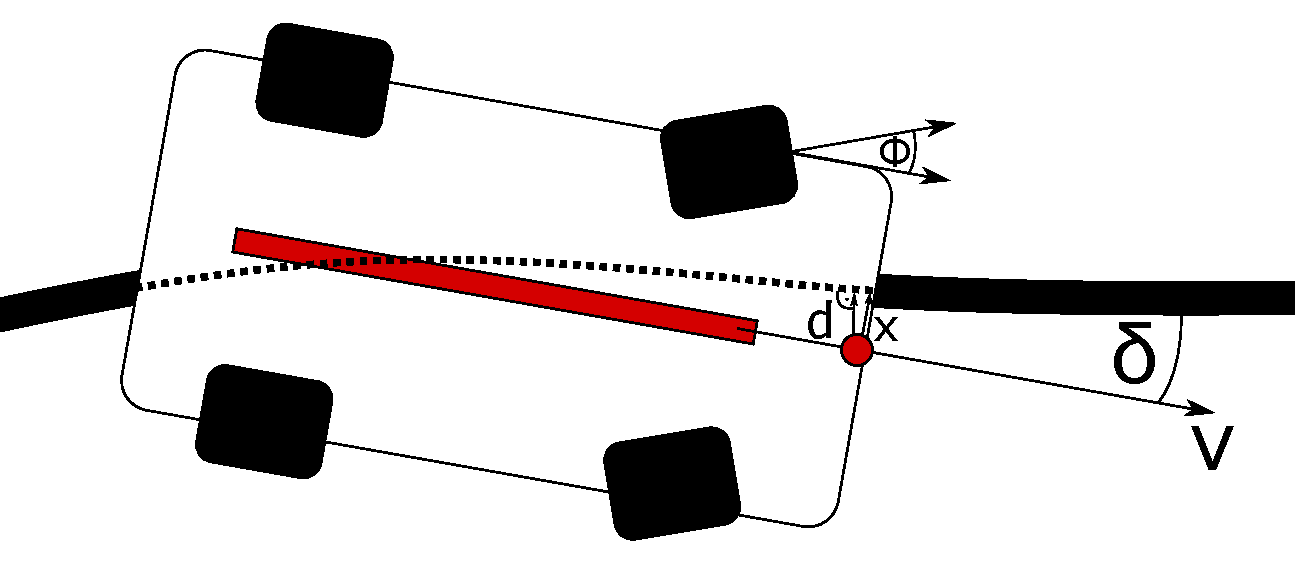
\includegraphics[width=0.9\linewidth]{img/cartop}
    \caption{A probléma sematikus ábrája felülnézetből}
    \label{fig:cartop}
\end{figure}

A \textbf{RobonAUT} verseny során egy olyan robot szoftverét és hardverét kell elkészíteni, amely lehetővé teszi a távirányítós autóból átalakított platformot, hogy egy ismeretlen pályán végighaladjon, és ott akadályokat teljesítsen, a szabályzatban meghatározott módon. A továbbiakban csak a szoftver környezettel foglalkozunk és feltételezzük, hogy megfelelő logikai jelek zajjal terhelten bár, de rendelkezésre állnak a szenzorokból, illetve az autó várakozásainknak megfelelően reagál a kimeneti jelekre, pl. a kormányszög beállítására.

A dokumentumban próbáljuk a szakirodalomban elterjedt jelrendszert alkalmazni, de az alábbi táblázat segítségével magyarázzuk a rendszeresen előforduló jelöléseket és összefüggéseket. Amennyiben valami hiányzik innen, az a szövegkörnyezetben kerül definiálásra.

\begin{center}
  \begin{tabular}{| c | p{0.8\linewidth} |}
\hline
    d & Pozícióhiba: Az első optikai szenzorsor középpontjának távolsága a vonaltól \\ \hline
    $ \delta $ & Szöghiba: Az első optikai szenzorsorra merőleges egyenes (középvonal) és a pályavonal érintője által bezárt szög \\ \hline
    $ \Phi $ & Kormányszög: A kerekek síkjainak a középvonallal bezárt szögeinek átlaga, Ackermann-kormányzás szerint \\
    \hline
    $ \kappa $ & A pálya pillanatnyi görbülete ($1/R$) \\ \hline
    x & Vonalpozíció: az első optikai szenzorsor által érzékelt vonalak középpontjának előjeles távolsága a szenzorsoron a közepponttól mérve. \\ \hline
    c & Vonalsebesség: x első deriváltja, a vonalpozíció mozgásának sebessége \\ \hline
    v & Sebesség: Az autó pillanatnyi sebessége a középvonal mentén \\
    \hline
  \end{tabular}
\end{center}

\section{Development Methods}

\paragraph{Classic Software Design Approach}

In every software development project, a visual sketch of the system is often created in order to aid the design process, and act as a visual guide during the documentation. However, implementing whatever design created earlier is not always trivial. The primary and most widespread embedded programming language, \textsf{C}, has been designed as a “Professional Programmers Language” \cite{essentialc}, and it supports only very basic syntax checks, but nothing ensures that the program will behave as the programmer intended. The designer must choose to take the risks of unexpected errors, or a thorough testing must be conducted in order to ensure the correct and reliable functioning of the system. While the testing of simple systems can be finished quickly, dangers arise when the same method is used in a large multi-developer project. Most of the industry have responded to this by scaling up the work force that gave birth to a number of strict project safety standards, internal regulations and coding guidelines \cite{misra}, and led to a huge amount of overhead in human labour in each software development project.

\paragraph{Model-Based Design}

As described earlier, the model-based design is based on solving the problems in a more visual environment. During the development, there is  limited connection between the designed software and the target hardware. Many of the solutions can be verified using the simulated model of the system, resulting in an accelerated development process\cite{locomotive}.
Due to the heavy reliance on abstract models and their connections, even if significant changes occur in the specifications, only minimal amount of modification is required to the code that formulates the final software. This advantage can not be over emphasized, because the final specifications of the system are rarely known, especially in prototype development.
Although it has its own limitations as well, model-based design relies on complex tools to do most of the work, and their operation and integration into an existing project is difficult and become less practical or limited because of the lack of sufficient support as well.

\paragraph{Background}

For the \textbf{RobonAUT 2014} contest, we used \textsf{MATLAB} and \textsf{Simulink} to implement the control system and the state machine. We chose the \textsf{MathWorks} product family, because \textsf{Simulink} has extensive support for model and simulation-based development, and allows the generation of \textsf{C} source code that can be later used on any hardware that is capable of running \textsf{FreeRTOS} or any other hard real-time operating systems. We have have used these technologies before successfully in industrial environment, which allowed us to follow out the concept.

\section{Model-based Design of the System}

% Contributions

Figure \ref{fig:architecture} shows the basic system connections and stages of deployment. A typical system designed in \textsf{MATLAB} can be divided to the following parts.

\begin{enumerate}
\item A \textsf{MATLAB} \textsf{Script} that defines the system model and computes the simulator and controller parameters.
\item Based on these parameters we can build the simulator and control software in \textsf{Simulink} that interact with each other.
\item If the system response in the simulation is correct, the controller is ready for code generation and field-testing.
\item The generated source code is invoked by the core operating system, the \textsf{FreeRTOS} in this case
\item All communication with the hardware in implemented by the Core.
\end{enumerate}

\begin{figure}[!ht]
    \centering
    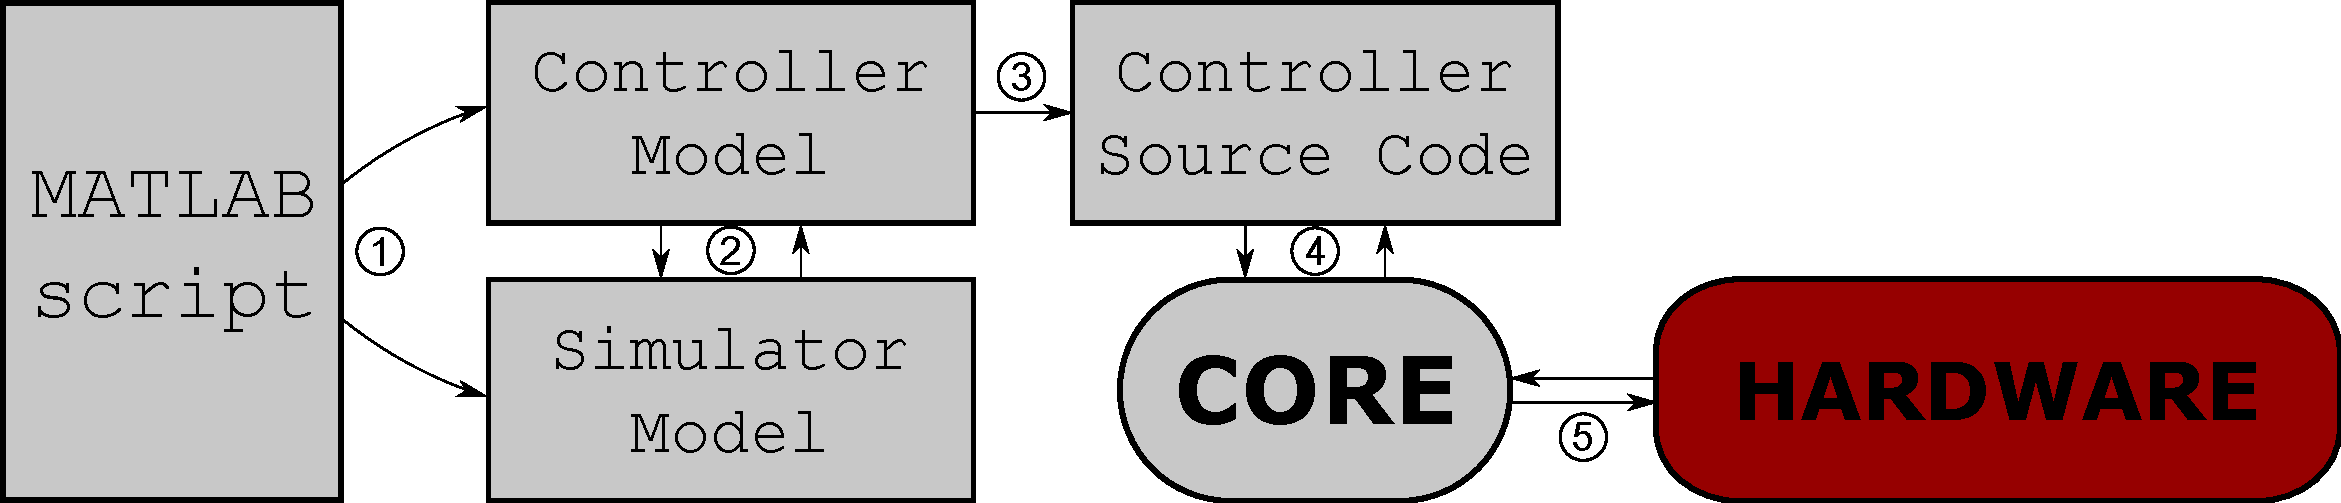
\includegraphics[width=0.7\linewidth]{img/architecture}
    \caption{Connections and dependencies}
    \label{fig:architecture}
\end{figure}

Although in most cases the core unit of a complex software will be an operating system, it is not mandatory. Therefore we use the \emph{Core} expression in this paper, but it refers to the \textsf{FreeRTOS} operating system in our case.

\subsection{Functional Description}

During the race, the track is marked by a dark line on light ground. The car follows this trail that guides it through certain checkpoints. In between there are obstacles that need to be passed in a specific way. Each obstacle is marked in a unique manner that allows the car to unambiguously determine, based on simple on-board sensors, which function it has to execute in the current segment.

The recommended sensor outfit\cite{sensors} is a number of optoelectronic sensors beneath the front axis or bumper of the car, and a couple of infrared proximity sensors at the front and two sides of the car. Certain teams extended this setup with a camera for image-recognition, a second optosensor array or ultrasound proximity sensors, but this paper will not consider any of these layouts.

\subsection{Building a Model}

The first step in model-based design is to create a model of the system, based on the functional description and known sensor fitting. To follow the line, the signals of the optical array must be processed and a control system must use this input to keep the car on the track. Let's define the following state variables:

\begin{center}
  \begin{tabular}{| c | p{0.7\linewidth} |}
\hline
    d & Position error: The shortest distance between the centre of the front optical array and the centre of the track \\ \hline
    $ \delta $ & Angular error: The angle between the centreline of the body and the tangent of the track \\ \hline
    $ \Phi $ & Steering angle: The effective steering angle, according to Ackermann-steering \\
    \hline
    $ \kappa $ & Current curvature of the track ($1/R$) \\ \hline
    x & Line position: the position of the track line along the front optical array \\ \hline
    c & Line speed: derivative of x, the change of the track line position \\ \hline
    v & Car speed: The current speed of the car along the centreline \\
    \hline
  \end{tabular}
\end{center}

Other variables with temporary significance might be defined in the text before their usage. Figure \ref{fig:cartop} helps to visualize the basic geometrics of the car, and the connections of the state variables.

\begin{figure}[!ht]
    \centering
    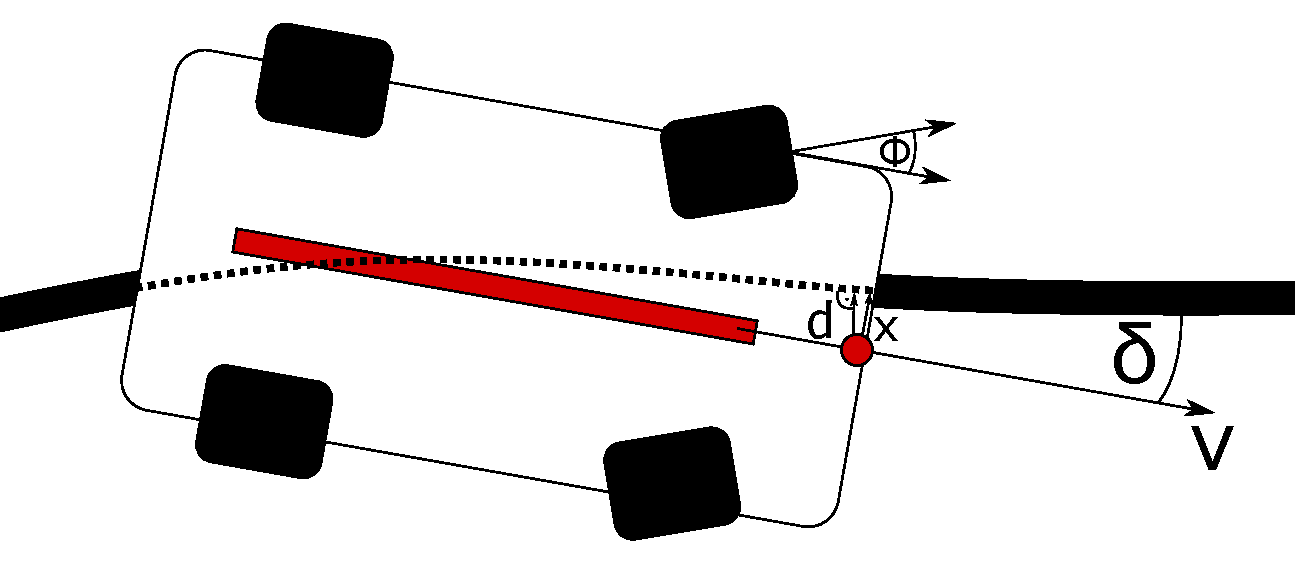
\includegraphics[width=0.7\linewidth]{img/cartop}
    \caption{System model}
    \label{fig:cartop}
\end{figure}

\paragraph{Formulating the System Model}

Knowing the dynamical system equations~(\ref{eq:of1}, \ref{eq:of2}), and parameters (L: wheelbase), we can formulate the \textbf{A} and \textbf{B}\footnote{The system is in discrete-time, but the continuous-time notation will be used throughout the paper, for better readability.} matrices based on their linear approximations in an equilibrium state $(d = 0; \delta = 0; v = 1)$ ~(\ref{eq:of3}).

\begin{align} 
    \dot{d} &= sin(\delta + \Phi) \cdot v  \label{eq:of1} \\ 
    \dot{\delta} &= \frac{v}{L} \cdot tan(\Phi) + \kappa \label{eq:of2}
\end{align}

% \begin{minipage}{0.45\linewidth}
%     \begin{align} \label{eq:of3}
%         \begin{bmatrix}
%                \dot{d} \\
%                \dot{\delta}
%         \end{bmatrix}
%         =
%         \begin{bmatrix}
%                0 & \delta \cdot v \\
%                0 & 0
%         \end{bmatrix}
%         %\cdot
%         \begin{bmatrix}
%                d \\
%                \delta
%         \end{bmatrix}
%      \end{align}
% \end{minipage}
% \begin{minipage}{0.45\linewidth}
%     \begin{align} \label{eq:of4}
%         \begin{bmatrix}
%                \dot{d} \\
%                \dot{\delta}
%         \end{bmatrix}
%         =
%         \begin{bmatrix}
%            0 & 0 \\
%            \frac{v}{L} & 1
%          \end{bmatrix}
%         %\cdot
%          \begin{bmatrix}
%                \Phi \\
%                \kappa
%         \end{bmatrix}
%      \end{align}
% \end{minipage}

    \begin{align} \label{eq:of3}
        \begin{bmatrix}
               \dot{d} \\
               \dot{\delta}
        \end{bmatrix}
        =
        \begin{bmatrix}
               0 & \delta \cdot v \\
               0 & 0
        \end{bmatrix}
        %\cdot
        \begin{bmatrix}
               d \\
               \delta
        \end{bmatrix}
		+
        \begin{bmatrix}
           0 & 0 \\
           \frac{v}{L} & 1
         \end{bmatrix}
        %\cdot
         \begin{bmatrix}
               \Phi \\
               \kappa
        \end{bmatrix}
     \end{align}

Instead of hard-coding the system matrices into the script, we can apply a different method that is nicer for the model-based approach, by using the \textsf{MATLAB} \textsf{Symbolic} \textsf{Toolbox}. This package allows the automatic generation of the Jacobi-matrices of the system, so the inputs are narrowed down to the system parameters and non-linear dynamic equations.
Furthermore, this way we can hold on to a lot more information that can later be used to generate a non-linear state observer, Extended Kalman Filter \cite{ekf}, or Hybrid Controller \cite{hybrid} for additional features in a complex system.
     
\paragraph{Control System}

Once an accurate system model is available, it's possible to formulate a controller. It's relatively easy to implement multiple controllers and compare them on the simulated system to determine, which would fit the robot the best.
Already knowing the state-space form of the system, a full-state feedback controller can be formulated quickly to stabilize the system. Using the Ackermann formula, we can obtain a suitable feedback matrix \textbf{K}, thus creating a stable new system with the feedback.

\begin{align}
	\underline{\dot{x}} = (A - BK) \cdot \underline{x}
\end{align}

\paragraph{Direct and Inverse Measurement Models}

Unfortunately, a full-state feedback loop can rarely be realized directly, hence the controller we have just created would not be able to control the actual system. Certain states can not be measured but only estimated by a state observer. The controller must be prepared to do that. Simulating the sensor readings based on the state variables is possible with the \emph{Direct measurement model}, while in order to estimate the states based on the sensor readings we need the \emph{Inverse measurement model}.

Knowing the geometrical layout of the car, the expected signals can be simulated using inverse geometric projection to the optosensor array:

\begin{align}
    x = \frac{d}{\cos(\delta)}
\end{align}

After the direct model has been determined, the inverse model can be formulated as well:

\begin{align}
    \hat{d} &= x \cdot \cos(\delta) \\
    \hat{c} &=\dot{x} \\
    \hat{\delta} &= \arctan \left(\frac{c}{v}\right) - \Phi
\end{align}

The direct model is usually part of the simulation only, however, it is possible to proof-check the sensor readings during run-time. This can be especially useful, if the states are estimated by sensor fusion. The inverse measurement model is always the first layer of the control loop, and it is rarely found in the simulated environment.

Note: $\delta$ can be directly measured if the robot is equipped with multiple optosensor arrays, but of course a different inverse measurement model is still necessary.

\subsection{Building the Simulation Environment}

When the system model and controller are available, it is time to build the simulation environment. In case of a simple system, at this point the controller could be implemented directly in \textsf{C}, but if the system is more complex, it is better practice to follow through the model-based design. To test the behaviour of the system, the controller and the simulator must be implemented in \textsf{Simulink} as well. Figure \ref{fig:simenvironment} shows the simulation-based development concept. Because the Controller model and the Controller source code are identical, the key is to design a simulator that is deceptively similar to the real system, from the point of view of the controller. This is the reason why Direct and Inverse Measurement (msment) models are required.

\begin{figure}[!ht]
    \centering
    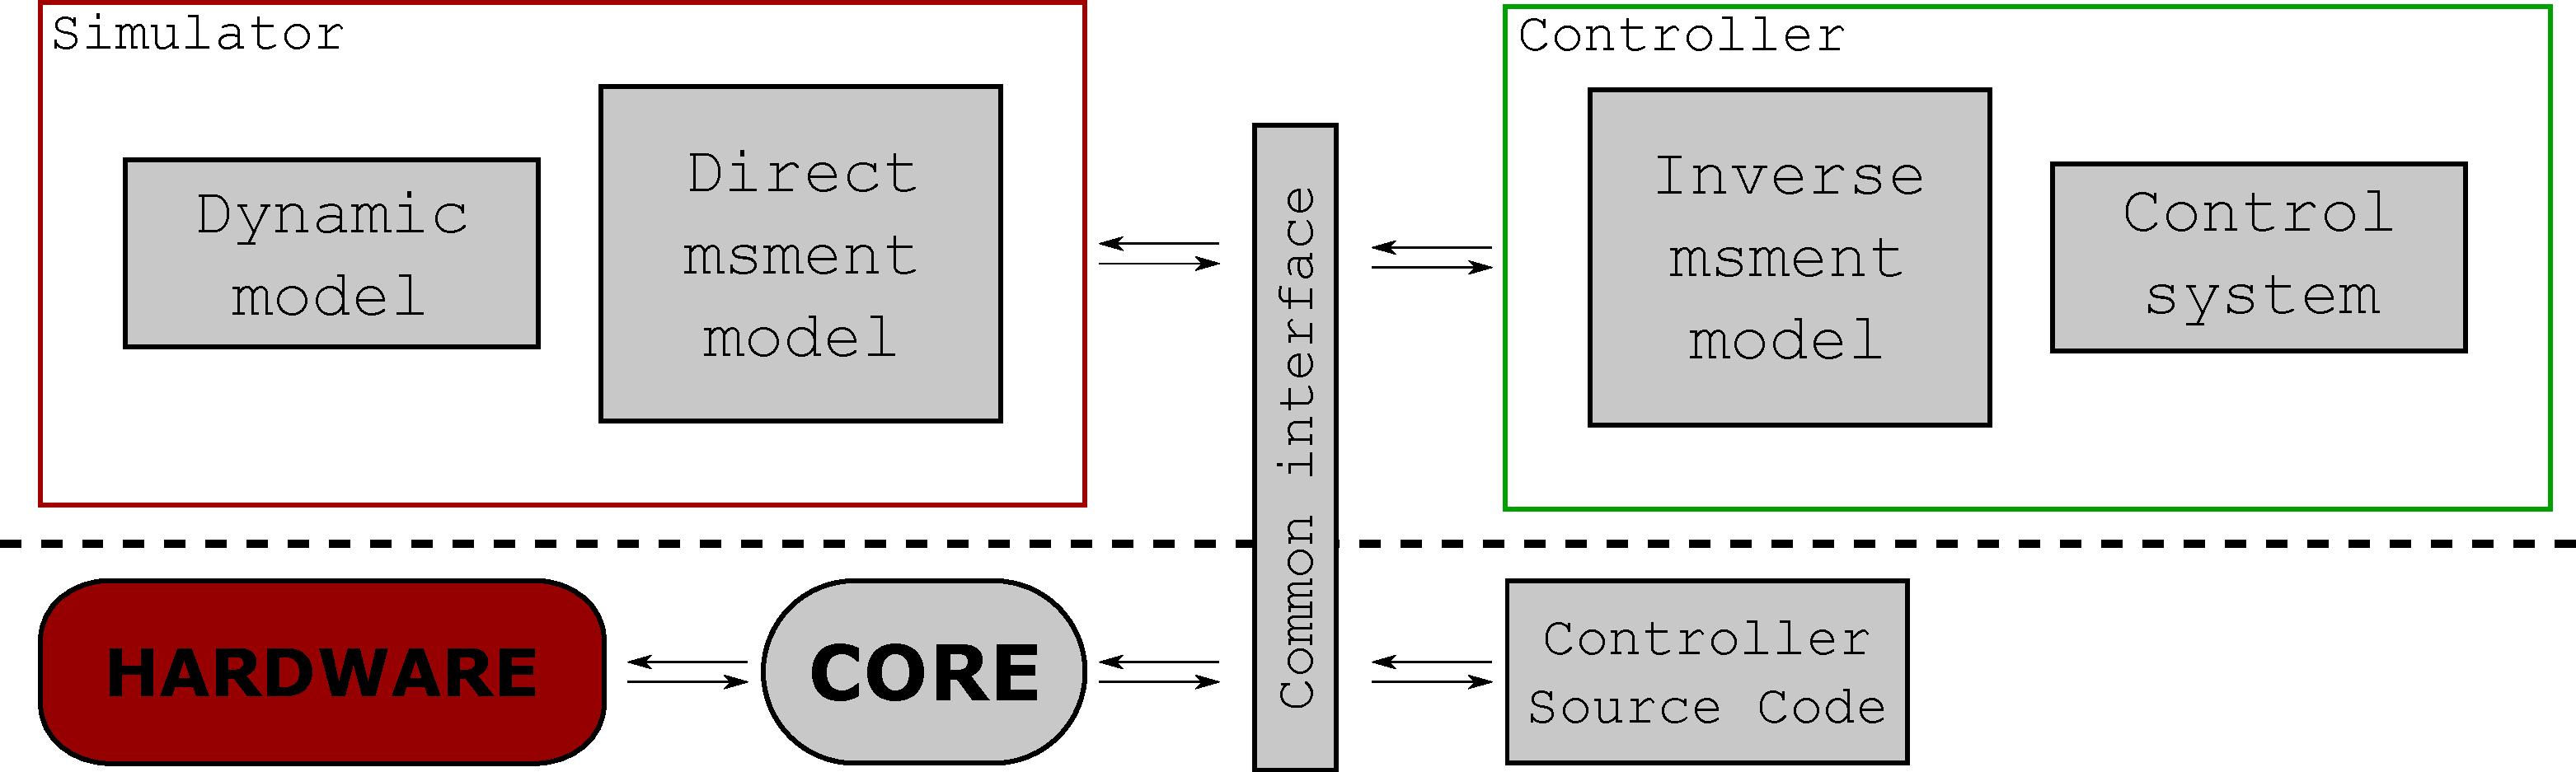
\includegraphics[width=0.7\linewidth]{img/simenvironment}
    \centering
    \caption{Simulation environment and analogy of deployment}
    \label{fig:simenvironment}
\end{figure}

Between the Simulator and Controller model, and between the Core and the Controller Source Code the actual sensor signals travel through a common interface, in the same form. The modules are interchangeable, without any functional loss. The modules themselves in the inside are working with the real (and estimated) state variables. The measurement models are mere encoding and decoding interfaces.

%Although \verb!MATLAB! is a dynamic typing language, it is good practice to fix the data type of the signals, especially if the software is developed for an embedded system. The default signal type is \emph{Double}, but it should be overridden to \emph{Single}, or \emph{Integer} to spare the limited processing capabilities of the system.

\subsection{Simulator Model}

The controller that was designed earlier is based on the linear approximation of the system, but the simulator must always represent the full non-linear system, or the whole model-based design effort is pointless. The system can be created with basic \textsf{Simulink} blocks. However, exploiting the technique described earlier to generate the Jacobi matrices of the system, we can use them directly to generate a full representation.

Figure \ref{fig:model} shows the simulation of the dynamics designed to test the control system (without inputs). A common programming analogy can describe how a discrete time \textsf{Simulink} \textsf{Model} works. The \textbf{States} block is the central element of the model, which stores the actual state variables. It is a \emph{storage unit}, which acts as a variable in this case. It outputs the value of the input of the previous time-step (which can be considered as a single execution of commands in a loop). The \textbf{Direct measurement model} simulates the sensor readings for the given state variables, in the same form as the expected inputs from the hardware, by generating the signal of each individual optosensor and putting them into a vector (same as a 1-dimensional array), just like as it is received from the Core.

Based on the system dynamics and the current value of the state variables, the states of the car can change. For example, a nonzero speed results in a change of traveled distance for the next time-step, even when there are no inputs to the system. The product of the state variables (\textbf{x}) and the system update matrix (\textbf{A}) results in a vector filled with the new states. In case of a linear system, \textbf{A} is constant. In case of a nonlinear system however, \textbf{A} depends on the current states. 

Consider the above example with nonzero speed (\textbf{v}), a straight track, the distance from the track (\textbf{d}) and angular deviation from the track ($\delta$). While the change of \textbf{d} is a linear function of \textbf{v}, it is also a trigonometric function of $\delta$. The resulting function is nonlinear, which means \textbf{A} is a nonlinear function of $\delta$. 

The Jacobian is a matrix of the first-order partial derivatives of the system \cite[p. 294]{jacobian}. It basically tells the effect of an individual state variable on the system. The summary of these effects result in the full system update.

\begin{align}
J =
		 \begin{bmatrix}
		  \frac{\partial F_1}{\partial x_1} & \cdots & \frac{\partial F_1}{\partial x_n} \\
		  \vdots  & \ddots & \vdots  \\
		  \frac{\partial F_n}{\partial x_1} & \cdots & \frac{\partial F_n}{\partial x_n}
		 \end{bmatrix}
\longrightarrow
 A_J =
		 \begin{bmatrix}
           \frac{\partial \dot{d}}{\partial d} & \frac{\partial \dot{d}}{\partial \delta} \\
           & \\
           \frac{\partial \dot{\delta}}{\partial d} & \frac{\partial \dot{\delta}}{\partial \delta}
         \end{bmatrix}
; \quad
B_J =
         \begin{bmatrix}
               \frac{\partial \dot{d}}{\partial \Phi} \\
               \\
               \frac{\partial \dot{\delta}}{\partial \Phi}
         \end{bmatrix}
\end{align}

If the system is linear, the elements of the matrix are constants. If the system in nonlinear, some elements of the matrix are functions of the state variables themselves.

\begin{figure}[!ht]
    \centering
    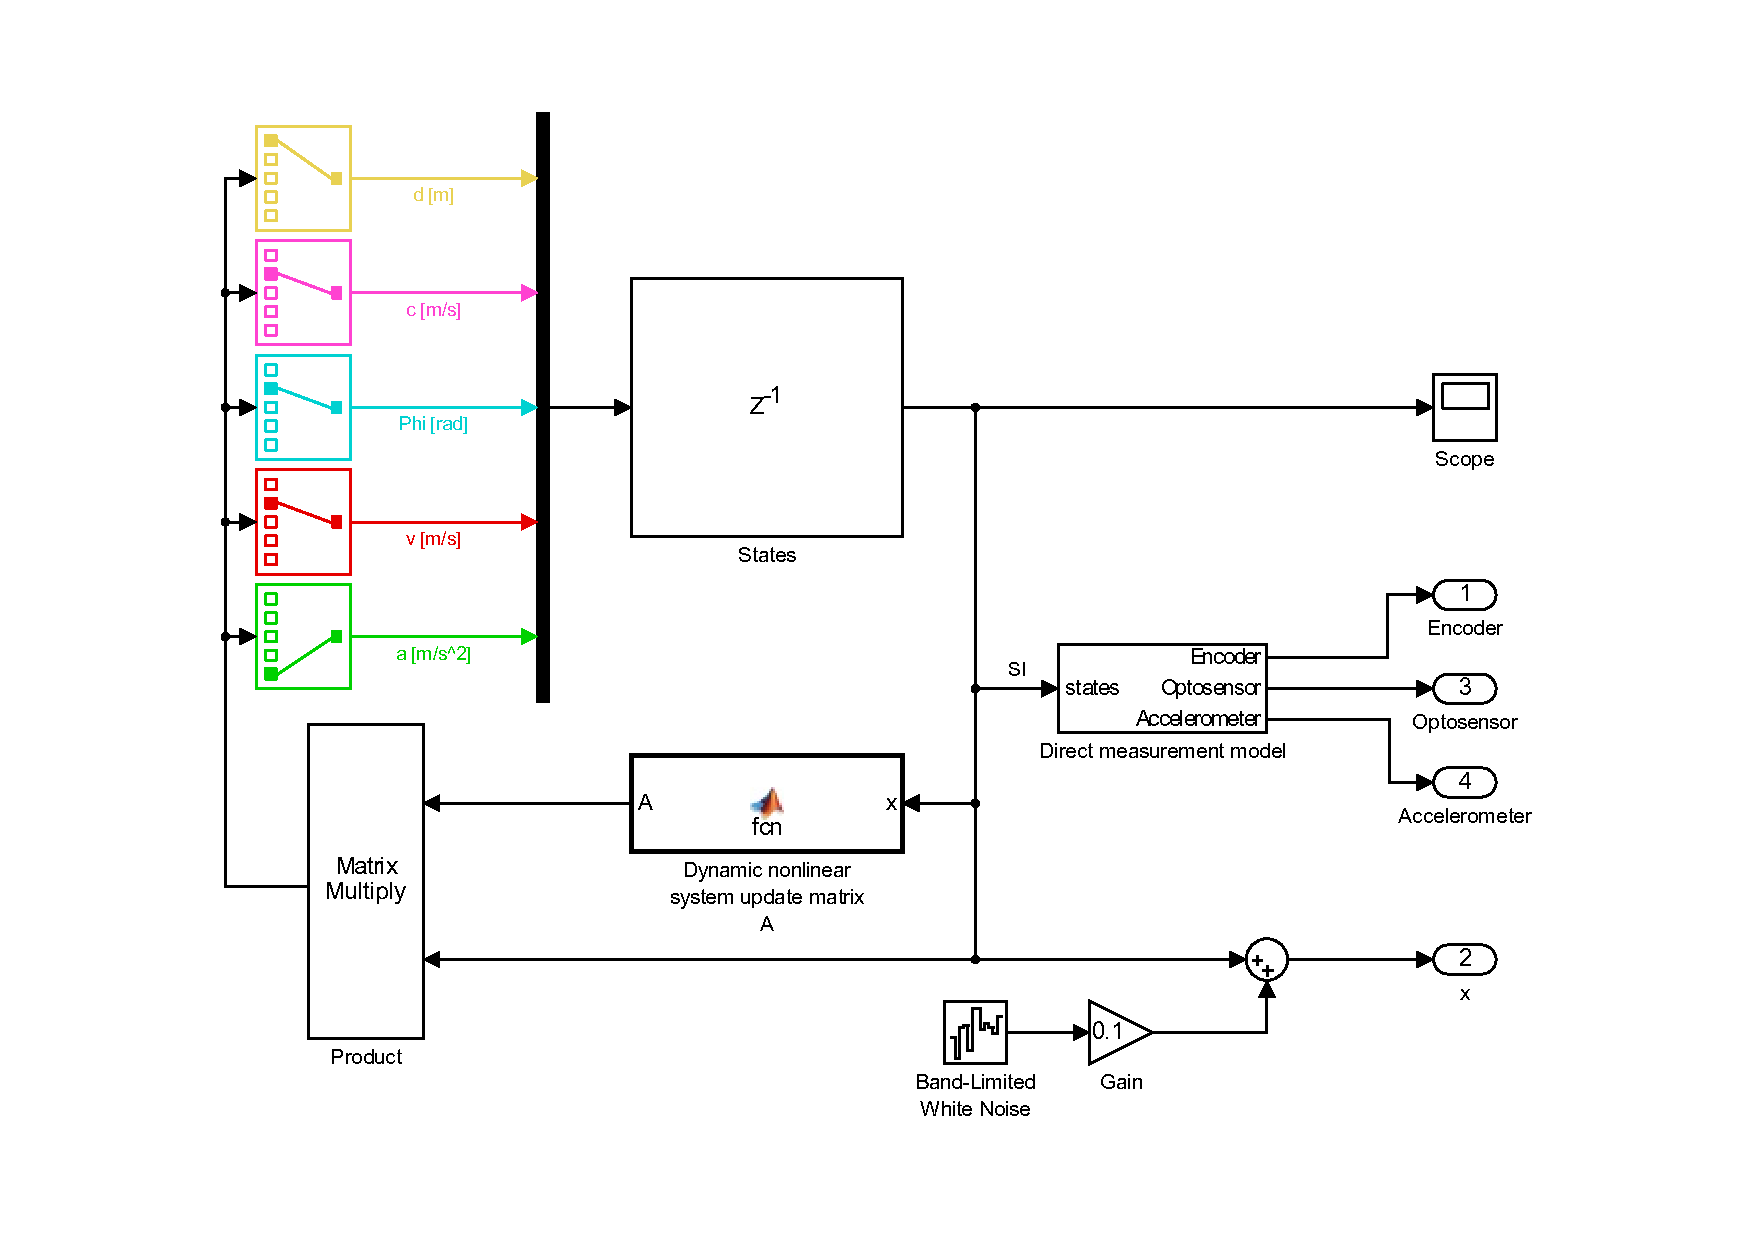
\includegraphics[width=0.7\linewidth]{img/sys}
    \centering
    \vspace{-20pt}
    \caption{Simulator model based on Jacobian matrices}
    \label{fig:model}
\end{figure}

The \textbf{Dynamic nonlinear system update matrix A} block contains a simple MATLAB script that builds the current system update matrix based on the Jacobian functions and the current states. Once we possess this, the system update phase can be executed just like in a linear case, with a matrix product. The resulting vector is the new set of state variables.

\subsection{Implementation of the Control System}

To describe the implementation of the entire control system is out of the scope of this paper, however, key aspects of the software will be highlighted. The visual development of the software requires a different way of thinking than working with traditional source code. Therefore, we encourage the reader to design his or her own control system, in order to get a first hand experience in model-based design.

\paragraph{Inverse Measurement Model}

The implementation of the inverse measurement model described earlier. During the race, multiple signals provide information about the track (optosensor array, side proximity sensors), therefore an inverse measurement model must be derived and realized for each of them, to provide the system states for the controller.

\paragraph{Controller}

Although basic processing might be required to enhance the raw signal quality before the inverse measurement model, any serious processing should be implemented in the next stage. Using model-based design, several controller implementations can be evaluated quickly by testing and comparing them using the dynamic simulation of the model. A word of caution though: an inferior simulator can negatively influence the results of the comparison. Always introduce the major physical limitations to the system, for example the non-zero transition time of the steering servo between states.

\subsection{High Level Control and State Machine}

\textsf{MATLAB} has an extension called \textsf{Stateflow} dedicated to the development of state machines. It integrates seamlessly with \textsf{Simulink} Models, and supports a wide range of features including subcharts, temporal logic and code generation as well, making it a very powerful tool. Figure \ref{fig:stateflow} shows the top layer of the state machine implementation of the obstacle course in \textsf{Stateflow}. It is primarily used to detect certain sections during the race based on the external signals, and take over the control of the car at some points to perform an action like the automated parking.

\begin{figure}[!ht]
    \centering
    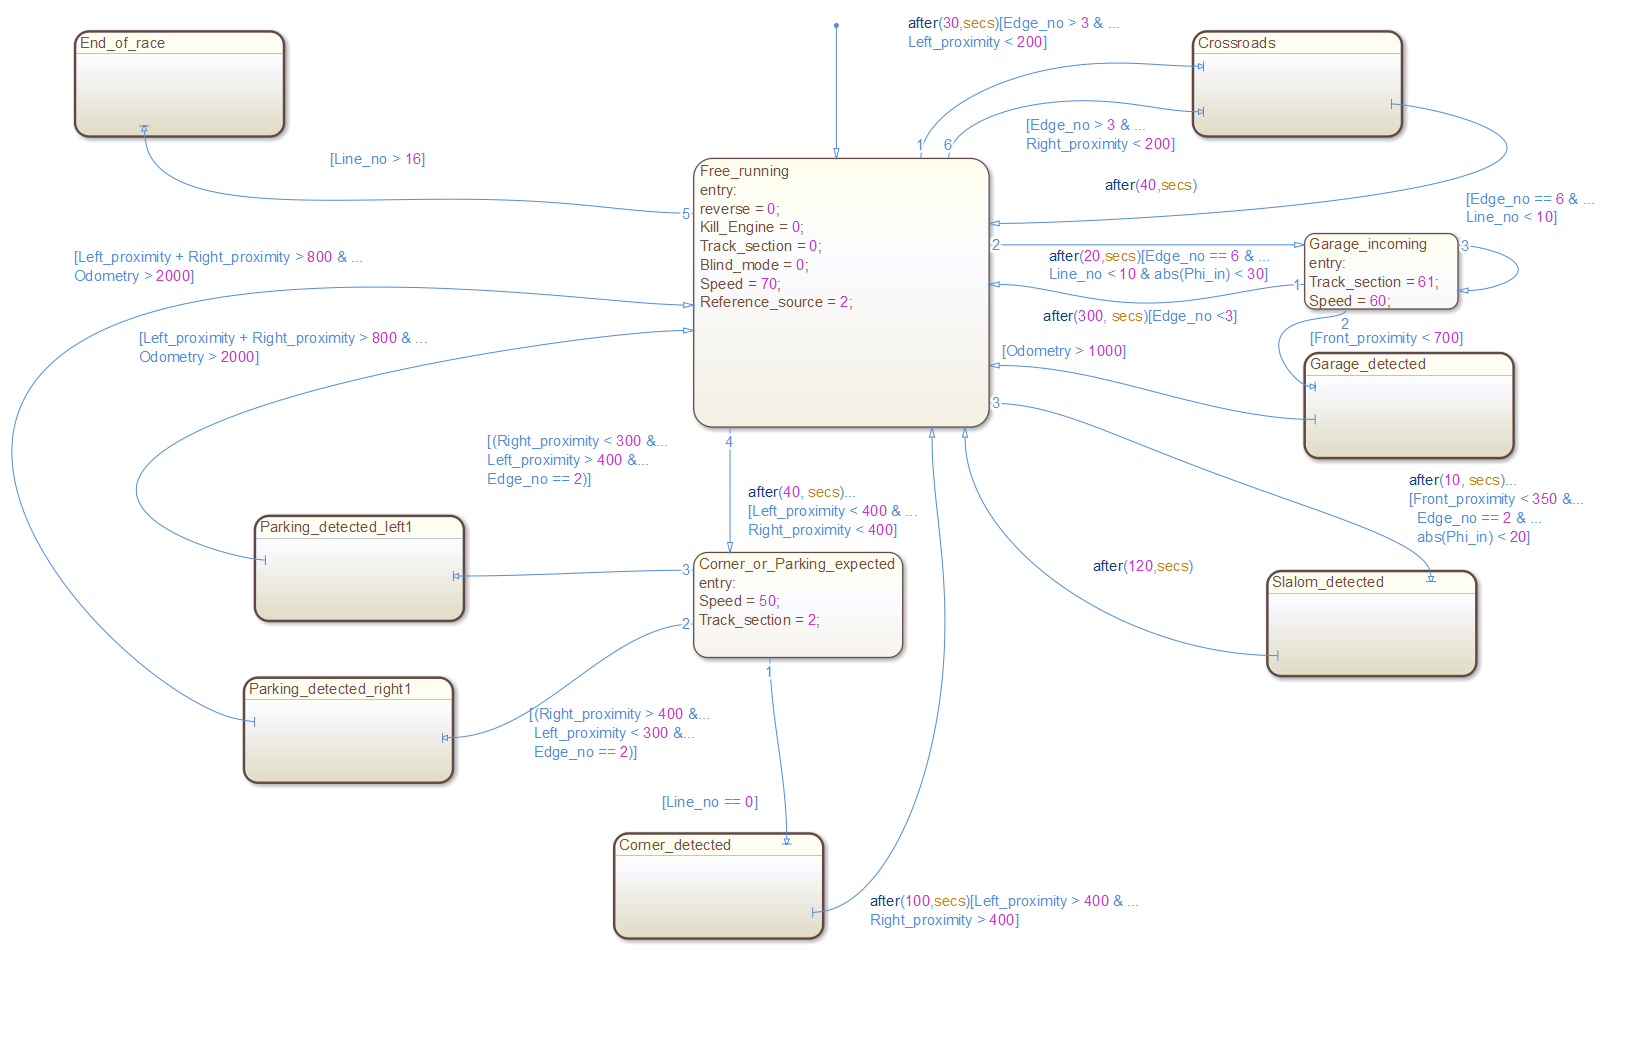
\includegraphics[width=0.7\linewidth]{img/stateflow}
    \centering
    \caption{State machine diagram of the obstacle course}
    \label{fig:stateflow}
\end{figure}







\section{Integration}
\label{sec:integration}

\subsection{Structure of the code}

If during the code generation \emph{Compact code placement} was used, only four files are generated:

\begin{itemize}

    \item "system\_name".c
    \item "system\_name".h
    \item rtwtypes.h
    \item ert\_main.c

\end{itemize}

In the following we assume that the name of the Controller block was "controlsystem".

\begin{figure}[!ht]
    \centering
    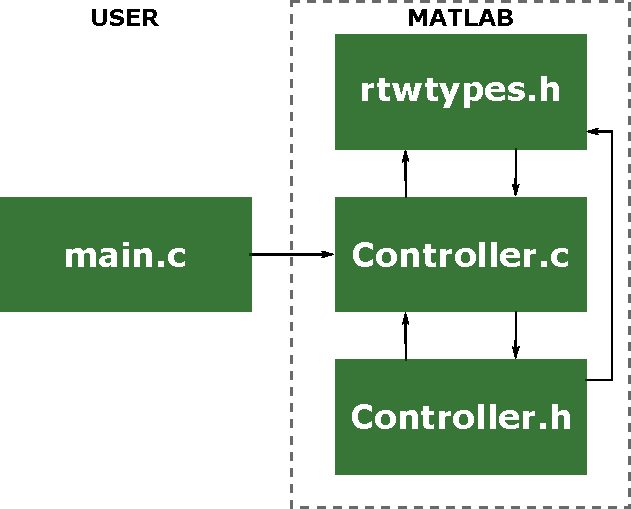
\includegraphics[width=0.6\linewidth]{img/rtw}
    \caption{Relationship of the generated files}
    \label{fig:rtw}
\end{figure}

The functions of the system are defined in the \textbf{controlsystem.c} and \textbf{controlsystem.h} files. The \textbf{rtwtypes.h} contains the unique type definitions of the code. The \textbf{ert\_main.c} is an exemplary main function that demonstrates the use of the others.

\subsection{Using the code}

The generated source code is functionally a perfect equivalent of the \verb!Simulink! model. The system can be initialized using the \emph{controlsystem\_initialize()} function. It sets the 0 time in the model and the outputs obtain their initial values. Communication with the system is only possible through a unique interface provided by the generated code. The inputs are handled by the \emph{controlsystem\_U struct}. It contains fields each corresponding to a system input, matching it's name and type. If the inputs are set, calling the \emph{controlsystem\_step()} function runs the model once, for the period of one time sample. The outputs are stored in a structure similar to the input storage, called \emph{controlsystem\_Y}.

\subsection{Deployment with FreeRTOS on STM32F4-Discovery Board}

As in many controlled processes, the timing of the controller program execution is crucial. Beside that it is also a time crucial task to process the I/O lines, convert the analog signals, and send status information to the supervisor computer over a wireless connection. It can be done with the integrated timer peripherals and with interrupt sequences, but the easiest way to handle a multi task problem like ours, is a \textbf{Real Time Operating System}. There are numerous implementation of these operating systems. We chose the FreeRTOS, which is a well known operating system in the industry, open-source, well documented and last but not least we have experience with it.

In our solution the FreeRTOS is responsible for the task scheduling, and provide a communication interface between the tasks. This way we can ensure that the sensors are read in the appropriate time, and the controller task will run in the specified time period. Also provides some useful tools to debug the application.
%Freertos mint Core mit csinál? (beszélget a hardverrel, szenzorokkal, aktuárotoknak küld beavatkozó jeleket)
%Miért jó? (gyors hozzáférés a szenzorokhoz, pontos ütemezés a controllernek)

Setting up the system is quite easy in this point. We only have to include the FreeRTOS source files into our project.\footnote{A detailed description is available for many processors in the FreeRTOS website: http://www.freertos.org/} The next step is to write some low level driver to read the sensors, and initialize the actuators so this way we can connect these to the control system. It is also necessary to set up the communication between the tasks, so we can read the state of the controller and the other tasks real time.
%Mit kellett csinálni, hogy működjön? (FreeRTOS-t feltenni rá (max 1 mondat, ebbe nem megyünk bele!), hardver jeleket kiolvasni C-vel, hogy oda tudjuk adni a controllernek, matlab-ot rákötni egy interrupt-ra)
%Még mit kell csinálni, hogy működjön?? Max 1-2 mondat már csak.

\section{Hardware-támogatás}

A MATLAB 2013b verziójától elérhető direkt hardware-támogatás az STM32F4 Discovery fejlesztőkártyához, melyet a MATLAB Hardware Support oldaláról tölthetünk le. A támogatás segítségével villámgyorsan tesztelhetjük az elkészített szoftvert, soros kábel segítségével pedig akár Processor-in-the-Loop tesztet is végrehajthatunk\cite[]{pilveri}.

\subsection{Gyors Prototípustervezés}

A RobonAUT elsősorban gyors prototípustervezési munkát igényel. Rövid idő alatt, minél hatékonyabb párhuzamosítással és a lehető legkevesebb teszteléssel kell sok funkcióval rendelkező, többé-kevésbé megbízható rendszert építeni. A magas és az alacsony szintű irányítás fejlesztése teljesen párhuzamosan zajlik, ha megfelelően kiaknázzuk a lehetőségeket.

\paragraph{Példa} Készítsünk Simulinkben egy LED-villogtató programot 5 perc alatt!

Miután feltelepítettük a support package-et\footnote{Ekkor indul a stopper}, hozzunk létre egy új Simulink modellt, majd húzzuk be az \textbf{Embedded Coder Support Package for STMF4-Discovery Board} library-ből a szükséges blokkokat. Az ábrán látható módon állítuk össze a kapcsolást, majd konfiguráljuk a modellt az 1. részben leírtakhoz hasonlóan, de most a \textbf{Code Generation} menüben \textbf{Target Hardware}-nek válasszuk az \verb!STM32F4-Discovery!-t, valamint ne csak kódot generáljunk (Pipa ki a \textbf{Generate code only} checkbox-ból).\footnote{Cheat sheet újoncoknak: A \texttt{Constant} blokk signal type-ját  \texttt{boolean}-re, a  \texttt{Pulse Generator} Pulse type-ját pedig  \texttt{Sample based}-re kell állítani. A blokkokról pedig senki sem tudja, hogy melyik almenüben vannak, érdemes használni a keresőt. Ne felejtsük el a GPIO blokkok konfigurálását sem! Ha semmiképpen sem akar működni, akkor a kész modell letölthető \href{http://www.mathworks.com/matlabcentral/fileexchange/45953-stm32f4-discovery-led-blinker}{\texttt{innen}}.}

\begin{figure}[!ht]
    \centering
    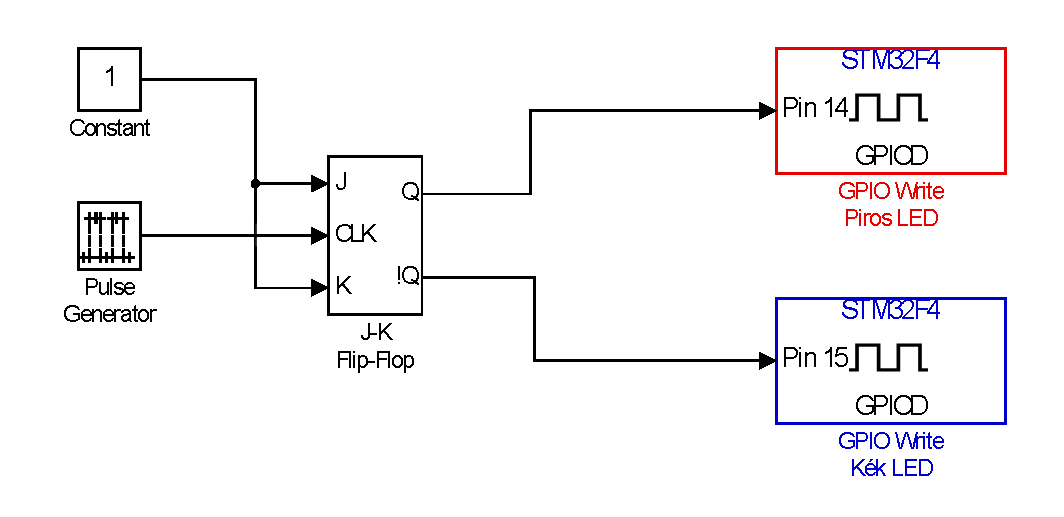
\includegraphics[width=0.9\linewidth]{img/stmblink}
    \caption{LED villogtató Simulink-modell}
    \label{fig:stmblink}
\end{figure}

A teljes rendszert a \textbf{Code} menü \textbf{C/C++ Code} menüpontjából tudjuk buildelni. Ha mindent jól csináltunk, a jutalmunk a végén egy \verb!.hex!, egy \verb!.elf! és egy \verb!.bin! file lesz a Working Directory-ben. Ezután az \texttt{STM ST-LINK Utility} segítségével felprogramozhatjuk a kártyát a generált fileok segítségével. Természetesen nem csak a ledeket tudjuk villogtatni, hanem az összes GPIO-t, gombot és analóg I/O-t kezelni tudjuk tetszőlegesen bonyolult modell köré építve. A GPIO Read és Write blokkok beállításához az \texttt{ST-Microelectronics} megfelelő segédletet nyújt\cite{usermanual}.

Hasonló elv alapján épült fel egy standard servo jeleket feldolgozó projekt is, melyet egy távirányítós autó végfokozatának PWM-es vezérlésére használtam.A Simulink modell szintén letölthető \href{http://www.mathworks.com/matlabcentral/fileexchange/46221-rc-car-control-with-stm32f4-discovery-programmed-by-matlab}{\texttt{innen}}, és mélyebb betekintést ad a modell alapú tervezés nyújtotta lehetőségekbe. Egy ilyen feladat elkészítése is inkább munkapercekben, mint -órákban mérhető.
Korábban említettük, hogy akár PIL tesztelésre is lehetőség van. Ebben a dokumentumban erre az alkalmazási területre nem térünk ki, de egy későbbi bővített kiadásban előfordulhat, ha igény mutatkozik a témára.


% An example of a floating figure using the graphicx package.
% Note that \label must occur AFTER (or within) \caption.
% For figures, \caption should occur after the \includegraphics.
% Note that IEEEtran v1.7 and later has special internal code that
% is designed to preserve the operation of \label within \caption
% even when the captionsoff option is in effect. However, because
% of issues like this, it may be the safest practice to put all your
% \label just after \caption rather than within \caption{}.
%
% Reminder: the "draftcls" or "draftclsnofoot", not "draft", class
% option should be used if it is desired that the figures are to be
% displayed while in draft mode.
%
%\begin{figure}[!t]
%\centering
%\includegraphics[width=2.5in]{myfigure}
% where an .eps filename suffix will be assumed under latex, 
% and a .pdf suffix will be assumed for pdflatex; or what has been declared
% via \DeclareGraphicsExtensions.
%\caption{Simulation Results}
%\label{fig_sim}
%\end{figure}

% Note that IEEE typically puts floats only at the top, even when this
% results in a large percentage of a column being occupied by floats.


% An example of a double column floating figure using two subfigures.
% (The subfig.sty package must be loaded for this to work.)
% The subfigure \label commands are set within each subfloat command, the
% \label for the overall figure must come after \caption.
% \hfil must be used as a separator to get equal spacing.
% The subfigure.sty package works much the same way, except \subfigure is
% used instead of \subfloat.
%
%\begin{figure*}[!t]
%\centerline{\subfloat[Case I]\includegraphics[width=2.5in]{subfigcase1}%
%\label{fig_first_case}}
%\hfil
%\subfloat[Case II]{\includegraphics[width=2.5in]{subfigcase2}%
%\label{fig_second_case}}}
%\caption{Simulation results}
%\label{fig_sim}
%\end{figure*}
%
% Note that often IEEE papers with subfigures do not employ subfigure
% captions (using the optional argument to \subfloat), but instead will
% reference/describe all of them (a), (b), etc., within the main caption.


% An example of a floating table. Note that, for IEEE style tables, the 
% \caption command should come BEFORE the table. Table text will default to
% \footnotesize as IEEE normally uses this smaller font for tables.
% The \label must come after \caption as always.
%
%\begin{table}[!t]
%% increase table row spacing, adjust to taste
%\renewcommand{\arraystretch}{1.3}
% if using array.sty, it might be a good idea to tweak the value of
% \extrarowheight as needed to properly center the text within the cells
%\caption{An Example of a Table}
%\label{table_example}
%\centering
%% Some packages, such as MDW tools, offer better commands for making tables
%% than the plain LaTeX2e tabular which is used here.
%\begin{tabular}{|c||c|}
%\hline
%One & Two\\
%\hline
%Three & Four\\
%\hline
%\end{tabular}
%\end{table}


% Note that IEEE does not put floats in the very first column - or typically
% anywhere on the first page for that matter. Also, in-text middle ("here")
% positioning is not used. Most IEEE journals/conferences use top floats
% exclusively. Note that, LaTeX2e, unlike IEEE journals/conferences, places
% footnotes above bottom floats. This can be corrected via the \fnbelowfloat
% command of the stfloats package.



\section{Results and future work}

The most important result is the successful application of the method. The system was designed and implemented in \verb!MATLAB!-generated code embedded into a \verb!FreeRTOS! Core, based on the methods described in this paper. Despite the odds and a challenging competition during the RobonAUT 2014, our car have scored a podium finish. It demonstrated complete reliability, though there have been performance issues in the faster sections, due to a flaw in the controller design. We plan to participate in the RobonAUT 2015 competition as well, and utilize the direct hardware support of \verb!MATLAB! for the \verb!STM32F4-Discovery!.

\section{Conclusion}






% conference papers do not normally have an appendix


% use section* for acknowledgement
\section*{Köszönet}
Szeretnénk köszönetet mondani konzulensünknek, Koszó Norbertnek a folyamatos segítségért, valamint az Automatizálási és Alkalmazott Informatikai Tanszék összes munkatársának, akiknek a RobonAUT versenyt köszönhetjük.






% trigger a \newpage just before the given reference
% number - used to balance the columns on the last page
% adjust value as needed - may need to be readjusted if
% the document is modified later
%\IEEEtriggeratref{8}
% The "triggered" command can be changed if desired:
%\IEEEtriggercmd{\enlargethispage{-5in}}

% references section

% can use a bibliography generated by BibTeX as a .bbl file
% BibTeX documentation can be easily obtained at:
% http://www.ctan.org/tex-archive/biblio/bibtex/contrib/doc/
% The IEEEtran BibTeX style support page is at:
% http://www.michaelshell.org/tex/ieeetran/bibtex/
%\bibliographystyle{IEEEtran}
% argument is your BibTeX string definitions and bibliography database(s)
%\bibliography{IEEEabrv,../bib/paper}
%
% <OR> manually copy in the resultant .bbl file
% set second argument of \begin to the number of references
% (used to reserve space for the reference number labels box)
\begin{thebibliography}{1}

\bibitem{szabtech}
Lantos-Kiss-Harmati: , \emph{Szabályozástechnika gyakorlatok}, \hskip 1em plus
  0.5em minus 0.4em\relax Budapest, BME-IIT, 2007.
  
\bibitem{usermanual}
STMicroelectronics: \href{http://www.st.com/st-web-ui/static/active/en/resource/technical/document/user_manual/DM00039084.pdf}{\emph{STM32F4-Discovery User Manual}, 2014 January}

\bibitem{pilveri}
MathWorks ST Discovery Board Support Documentation Examples: \emph{Code Verification and Validation with PIL and External Mode}


\end{thebibliography}




% that's all folks
\end{document}


